\documentclass[a4paper]{article}   % list options between brackets
\usepackage{CJK}
\usepackage{fullpage}
\usepackage{graphicx}
\usepackage{graphics}
\usepackage{tabularx}
\usepackage{listings}
\usepackage{rotating}
\usepackage{setspace}
\usepackage{amsmath}
\usepackage{caption}
\usepackage{xcolor}
\usepackage{cite}

\lstset{numbers=left, numberstyle=\small, frame=shadowbox,
xleftmargin=2em,xrightmargin=2em, aboveskip=1em, breaklines,
extendedchars=false, tabsize=4, basicstyle=\linespread{1.0}\ttfamily,
commentstyle=\ttfamily\normal\small, keywordstyle=\color{blue!70}
}

% type user-defined commands here


\begin{document}
\begin{CJK}{UTF8}{gbsn}
\begin{spacing}{1.2}

\title{High Performance Computing\\ Homework 2\\ Report}
\author{Peiyun Hu, 2010011297\\ Department of Computer Science \& Technology}
\maketitle

\section{A parallel algorithm for a limited Lx=b}
\subsection{Description}
Please refer to the homework file. 
\subsection{Answer}
%The Input and Output information is shown below in the Table \ref{table:io_1}.
%\begin{center}
%\label{table:io_1}
%\begin{tabular}{c|c|c|c}
%
% Task & Input & Output & Subtask:(i, j) \\ 
% $t_0$ & $\emptyset$ & $x_0$ \\ 
% $t_1$ & $x_0$ & $b_0$, $x_1$ \\ 
% $t_2$ & $x_0$, $x_1$ & $b_2$, $x_2$ \\ 
% $\dots$ & $\dots$ & $\dots$ \\ 
% $t_{n-1}$ & $x_0 \dots x_{n-2}$ & $b_{n-1}, x_{n-1}$ \\ 
%
%\end{tabular} 
%\end{center}
Actually, there is an order that must be followed. For $x_i$ is determined by $x_{i-1} (i>=0) $, $x_i$ should wait until new $x_{i-1}$ is calculated. 



So, the dependencies graph i actually a complete graph, which is shown as Figure~\ref{myfig}. And it is really embarrassing to execute in parallel. However, there is another way to think over this program. And when the definition of task changed, this program could be paralleled better. Specifically, we define (i, j) a task.

\begin{figure}[htbp]
\centering
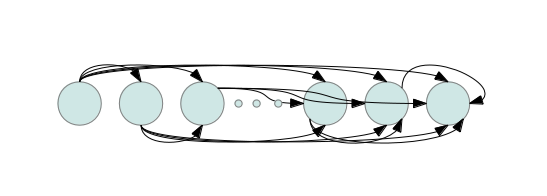
\includegraphics[scale=0.5]{dependencies.png} 
\caption{Dependencies}\label{myfig}
\end{figure}

The order could be shown in the Table \ref{tbl:ideal_order}.

\begin{table}[htbp]
\centering
\begin{tabular}{|c|c|c|c|c|c|c|c|c|}
\hline
 t & 1 & 2 & 3 & 4 & 5 & \dots & m-1 & m \\ 
  & (0, ) &  &  &  &  & \dots &  &  \\ 
  &  & (1,0) &  &  &  & \dots &  &  \\ 
  &  & (2,0) &   (2,1) &  &  & \dots & &  \\
  &  & (3,0) &  (3,1) & (3,2) &  &\dots &  &\\
  &  & \dots &  \dots & \dots & \dots & \dots &  &  \\
  &  & (n-1,0) &  (n-1,1) & (n-1,2)& (n-1,3) & \dots &(n-1, n-2) &  \\
  &  & (n,0) &  (n,1)& (n,2) & (n,3) & \dots &(n, n-2) & (n,n-1) \\
\hline 
\end{tabular}
\caption{Ideal order of execution}
\label{tbl:ideal_order}
\end{table} 

As is shown in the table above, we could ideally infer that we could solve this problem in 
 $n+1 $ column time, only if the number of processors is more than that of rows. If so, each column will cost almost the same time. While, especially when the size of matrix is very enormous, we should execute them in a specified order.
 
When considering the order or execution, we should notice that even if we decompose the task into smaller granularity, there are still dependencies among them. To put it in another way, in order to follow the dependencies, we assign the tasks levels of priority. For task (i, j), unless $x_j$ is worked out, it should never be executed. Also, the executed order of tasks ($i_1$, j), ($i_2$, j), \dots, ($i_k$, j), should be in ascending order of $i$, that is to say, the smaller i is, the task should be executed earlier. Because the smaller i is, strictly, the possibility of augment of available $x_i$ is higher. In order to expand available tasks, tasks that have smaller i are executed first. 

And there is an specific example shown in \ref{example}.

%Because I could not figure out what a dependence graph and a task interaction graph look like, I drew a table instead. And each column is directly dependent on the first element of its previous row. 

%It is a little embarassing for the dependences, especially when there is not that much processors. But there do exist some decent algorithms to solve this. For example, owing to the dependences, we could assign each (i, j) (could be a subtask) a priority level.  And the priority of each subtask is lower than  subtask which determines it, and higher than which it determines. What is more, we could let (i, i-1) be done while it is available, and in this way, we could overlap the executing time of (i, i-1) with that of \{(i, i-2), (i+1, i-2), \dots , (n, i-2)\} in order to expand available columns more quickly. 

\subsection{An example} \label{example}

If n = 256, and only 16 processors, we could create a working pool which looks like a stack. Each time when we pop out task like (i, i-1), we push in \{ (i+1, n), (i+1, n-1), \dots, (i+1, i-1) \} in successively. In each period, we pop out up to 16 tasks to execute, then push in if needed. There is a master processor to allocate tasks to other processors, and other processors wait for tasks. After every period, the sequence of x should be updated in each processor.(Indeed, I think it should be each 'thread' instead of each 'processor'.)

In this way, the tasks in the stack are all available to be allocated and executed. 

\section{Simplified Bucket-Sort\label{problem2}}
\subsection{Description}
Please refer to the homework file. 

\subsection{Answer}
\subsubsection{Analysis} \label{analysis_problem2}
The bucket-sort problem contains the iteration of array A and buckets. So to balance the workload of two aspects, we have two strategies. 

\subsubsection{Partition the Input Data} \label{first_method_problem2}
The strategy of decomposition is to divide input data into p parts averagely, that is to say, each part has roughly $\frac{p}{n}$ elements. Then every process works as a sequential task. Finally, communication  should be done to gather results to one process, then the 'master' process print the results out . 

\subsubsection{Partition the Output Data} \label{second_method_problem2}
Aside from the strategy above, we develop another which is focued on the workload of buckets' iteration. There could be a 'master' process, which is denoted $p_0$. The iteration of array is done in $p_0$, and it will get the value of A[i], then put the index of it into the correponding bucket. When assignment is done, including $p_0$, each processor is allocated with several buckets averagely, which is in consecutive order of buckets' indices. Then every process do the iteration of buckets and fetch indices from nonempty buckets to fill up a new sorteddd array. Finally, after filling up inside each process, $p_0$ starts to collect results and print them out. 

\section{More about Problem \ref{problem2}.}
\subsection{Description}
Please refer to the homework file. 
\subsection{Answer}
It depends which decomposition leads to a better parallel algorithm, as is stated in \ref{analysis_problem2}. 
\paragraph*{Specifically}
When n $\gg$ r, which means that iteration of array will cost much more than that of buckets. So the method in \ref{first_method_problem2} will outperform the one described in \ref{second_method_problem2}. When n $\ll$ r, and the cost of iterating buckets will outnumber that of iterating the array. In this case, the method in \ref{first_method_problem2} is more appropriate. When the gap between n and r is small, there would be little difference in the level of algorithm. 
\paragraph*{Moreover} When size of both array and buckets are huge, actually, both two strategies could be leveraged to fulfill the task. That is to say, iteration of array and buckets are done in parallel way. 

\bibliographystyle{plain}
\bibliography{bibitex}

\appendix
\section*{Appendix}


\end{spacing}
\end{CJK}
\end{document}
